\tikzset{every picture/.style={line width=0.75pt}} %set default line width to 0.75pt        
\begin{center}
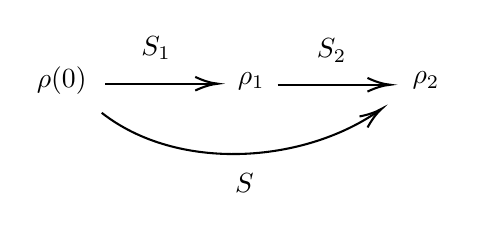
\begin{tikzpicture}[x=0.75pt,y=0.75pt,yscale=-1,xscale=1]
%uncomment if require: \path (0,300); %set diagram left start at 0, and has height of 300

%Straight Lines [id:da4078450591380367] 
\draw    (186,145.5) -- (238.25,145.5) ;
\draw [shift={(240.25,145.5)}, rotate = 180] [color={rgb, 255:red, 0; green, 0; blue, 0 }  ][line width=0.75]    (10.93,-3.29) .. controls (6.95,-1.4) and (3.31,-0.3) .. (0,0) .. controls (3.31,0.3) and (6.95,1.4) .. (10.93,3.29)   ;

%Straight Lines [id:da9736233485654777] 
\draw    (269,146) -- (321.25,146) ;
\draw [shift={(323.25,146)}, rotate = 180] [color={rgb, 255:red, 0; green, 0; blue, 0 }  ][line width=0.75]    (10.93,-3.29) .. controls (6.95,-1.4) and (3.31,-0.3) .. (0,0) .. controls (3.31,0.3) and (6.95,1.4) .. (10.93,3.29)   ;

%Curve Lines [id:da5450320200035714] 
\draw    (184.25,159.5) .. controls (220.88,188.21) and (281.52,184.09) .. (318.15,158.29) ;
\draw [shift={(319.25,157.5)}, rotate = 504.02] [color={rgb, 255:red, 0; green, 0; blue, 0 }  ][line width=0.75]    (10.93,-3.29) .. controls (6.95,-1.4) and (3.31,-0.3) .. (0,0) .. controls (3.31,0.3) and (6.95,1.4) .. (10.93,3.29)   ;


% Text Node
\draw (165,143.83) node   {$\rho ( 0)$};
% Text Node
\draw (256.33,144.17) node   {$\rho _{1}$};
% Text Node
\draw (340.5,144) node   {$\rho _{2}$};
% Text Node
\draw (253,193.5) node   {$S$};
% Text Node
\draw (210.5,128.5) node   {$S_{1}$};
% Text Node
\draw (295,129.5) node   {$S_{2}$};


\end{tikzpicture}
\end{center}